% !TeX spellcheck = cs_CZ
{\tikzset{external/prefix={tikz/FYZII/}}
 \tikzset{external/figure name/.add={ch28_}{}}
%---------------------------------------------------------------------------------------------------
% file fey2ch28.tex
%---------------------------------------------------------------------------------------------------
%=========================== Kapitola Elektromagnetická hmotnost ===================================
\chapter{Elektromagnetická hmotnost}\label{fyz:IIchapXXIIX}
\minitoc
  \section{Energie pole bodového náboje}\label{fyz:IIchapXXIIXsecI}
  \section{Hybnost pole pohybujícího se náboje}\label{fyz:IIchapXXIIXsecII}
  \section{Elektromagnetická hmotnost}\label{fyz:IIchapXXIIXsecIII}
  \section{Síla, kterou elektron působí sám na sebe}\label{fyz:IIchapXXIIXsecIV}
  \section{Pokusy o modifikaci Maxwellovy teorie}\label{fyz:IIchapXXIIXsecV}
  \section{Pole jaderných sil}\label{fyz:IIchapXXIIXsecVI}
  \section{Příklady a cvičení}\label{fyz:IIchapXXIIXsecVII}

    \begin{figure}[ht!] %\ref{fyz_fig617}
      \centering
      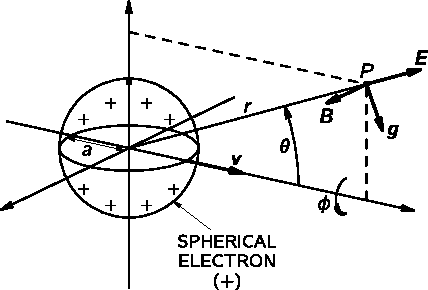
\includegraphics[width=0.7\linewidth]{fyz_fig617.pdf}
      \caption{
               (\cite[s.~707]{Feynman02})}
      \label{fyz_fig617}
    \end{figure}

    \begin{figure}[ht!] %\ref{fyz_fig618}
      \centering
      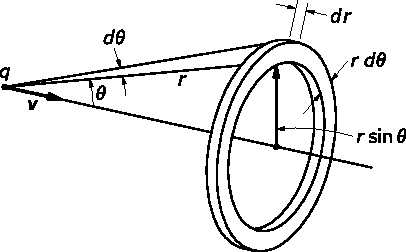
\includegraphics[width=0.7\linewidth]{fyz_fig618.pdf}
      \caption{
               (\cite[s.~707]{Feynman02})}
      \label{fyz_fig618}
    \end{figure}

    \begin{figure}[ht!]
      \centering
      \begin{tabular}{ccc}
        \subfloat[ ]{\label{fyz_fig619a}
          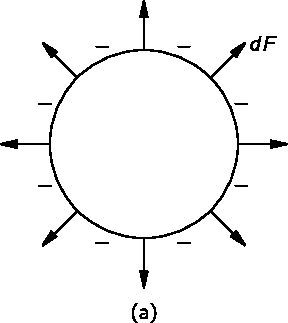
\includegraphics[width=0.3\linewidth]{fyz_fig619a.pdf}}               &
        \subfloat[ ]{\label{fyz_fig619b}
          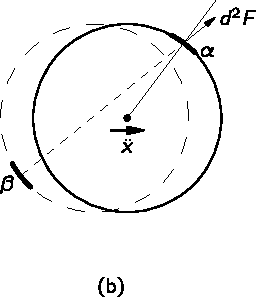
\includegraphics[width=0.3\linewidth]{fyz_fig619b.pdf}}               &
        \subfloat[ ]{\label{fyz_fig619c}
          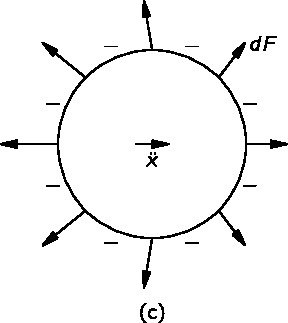
\includegraphics[width=0.3\linewidth]{fyz_fig619c.pdf}}
      \end{tabular}
      \label{fyz_fig619}
      \caption{
               (\cite[s.~748]{Feynman02})}
    \end{figure}

    \begin{figure}[ht!] %\ref{fyz_fig620}
      \centering
      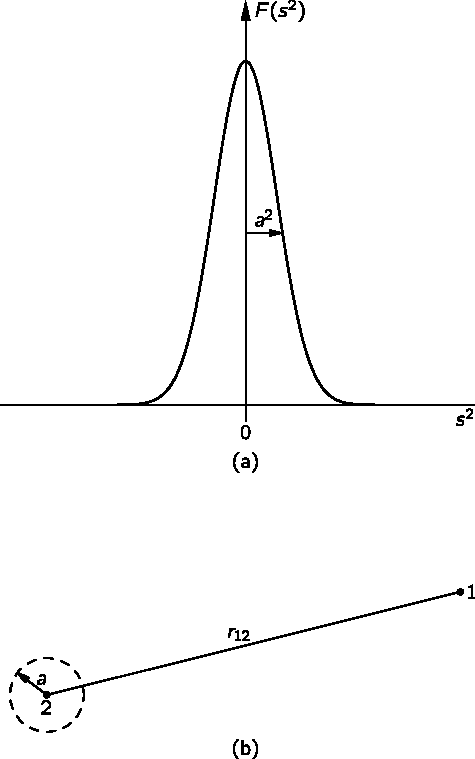
\includegraphics[width=0.7\linewidth]{fyz_fig620.pdf}
      \caption{
               (\cite[s.~707]{Feynman02})}
      \label{fyz_fig620}
    \end{figure}

    \begin{figure}[ht!] %\ref{fyz_fig621}
      \centering
      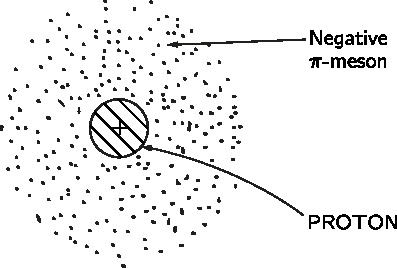
\includegraphics[width=0.7\linewidth]{fyz_fig621.pdf}
      \caption{
               (\cite[s.~707]{Feynman02})}
      \label{fyz_fig621}
    \end{figure}

    \begin{figure}[ht!] %\ref{fyz_fig622}
      \centering
      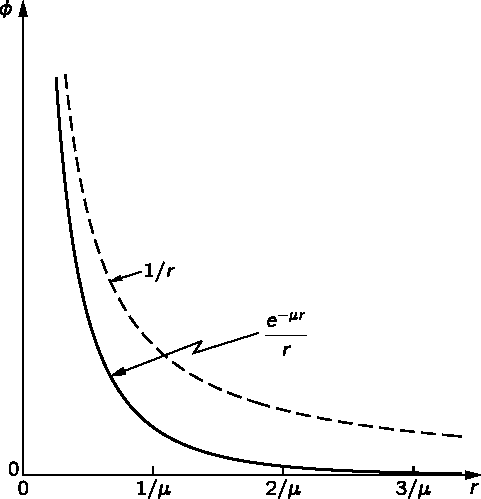
\includegraphics[width=0.7\linewidth]{fyz_fig622.pdf}
      \caption{
               (\cite[s.~707]{Feynman02})}
      \label{fyz_fig622}
    \end{figure}


















} %tikzset
%---------------------------------------------------------------------------------------------------
\printbibliography[title={Seznam literatury},heading=subbibliography]
\addcontentsline{toc}{section}{Seznam literatury}